\documentclass{article}
\usepackage[utf8]{inputenc}
\usepackage[T1,OT1]{fontenc}
\usepackage{lmodern}
\usepackage{listings}
\usepackage{minted}
\usepackage{amsmath}
\usepackage[none]{hyphenat}
\usepackage{multicol}
\usepackage{pgfplots}
\usepackage{makecell}

\title{Intelligent Data Mining - Exercise 4}
\author{\fontencoding{T1}\selectfont Michael Debono Mrđen}
\date{14 November 2017}

\begin{document}

\maketitle

\section{Assignment 1: Minhashing}
\renewcommand{\labelenumi}{\alph{enumi}.}
\renewcommand{\labelenumii}{(\alph{enumii})}

\begin{enumerate}
\item{Compute the minhash signature for each column if we use the following three hash functions:
	\begin{itemize}
		\item $h_1(x)=2x+1\mod{6}$
		\item $h_2(x)=3x+2\mod{6}$
		\item $h_3(x)=5x+2\mod{6}$
	\end{itemize}

\begin{center}
\begin{tabular}{ c | c | c | c | c || c | c | c }
	Element & $S_1$ & $S_2$ & $S_3$ & $S_4$ & $h_1$ & $h_2$ & $h_3$ \\ \hline\hline
	0       & 0     & 1     & 0     & 1     & 1     & 2     & 2     \\
	1       & 0     & 1     & 0     & 0     & 3     & 5     & 1     \\
	2       & 1     & 0     & 0     & 1     & 5     & 2     & 0     \\
	3       & 0     & 0     & 1     & 0     & 1     & 5     & 5     \\
	4       & 0     & 0     & 1     & 1     & 3     & 2     & 4     \\
	5       & 1     & 0     & 0     & 0     & 5     & 5     & 3
\end{tabular}
\end{center}
	
}
\item{Which of these hash functions are true permutations?
	
Only $h_3$ is a true permutation as it defines different hashes for all available elements.
}
\item{How close are the estimated Jaccard similarities (based on the minhashes) for the six pairs of columns to the true Jaccard similarities.

Signature matrix computation:
\begin{center}
	\begin{equation}
	\begin{tabular}{ c || c | c | c | c } \label{1}
		      & $S_1$    & $S_2$    & $S_3$    & $S_4$    \\ \hline
		$h_1$ & $\infty$ & $\infty$ & $\infty$ & $\infty$ \\
		$h_2$ & $\infty$ & $\infty$ & $\infty$ & $\infty$ \\
		$h_3$ & $\infty$ & $\infty$ & $\infty$ & $\infty$
	\end{tabular}
	\end{equation}

	\begin{equation}
	\begin{tabular}{ c || c | c | c | c }
		      & $S_1$    & $S_2$ & $S_3$    & $S_4$ \\ \hline
		$h_1$ & $\infty$ & 1     & $\infty$ & 1     \\
		$h_2$ & $\infty$ & 2     & $\infty$ & 2     \\
		$h_3$ & $\infty$ & 2     & $\infty$ & 2
	\end{tabular}
	\end{equation}
	
	\begin{equation}
	\begin{tabular}{ c || c | c | c | c }
		      & $S_1$    & $S_2$ & $S_3$    & $S_4$ \\ \hline
		$h_1$ & $\infty$ & 1     & $\infty$ & 1     \\
		$h_2$ & $\infty$ & 2     & $\infty$ & 2     \\
		$h_3$ & $\infty$ & 1     & $\infty$ & 2
	\end{tabular}
	\end{equation}
	
	\begin{equation}
	\begin{tabular}{ c || c | c | c | c }
		      & $S_1$ & $S_2$ & $S_3$    & $S_4$ \\ \hline
		$h_1$ & 5     & 1     & $\infty$ & 1     \\
		$h_2$ & 2     & 2     & $\infty$ & 2     \\
		$h_3$ & 0     & 1     & $\infty$ & 0
	\end{tabular}
	\end{equation}
	
	\begin{equation}
	\begin{tabular}{ c || c | c | c | c }
		      & $S_1$ & $S_2$ & $S_3$ & $S_4$ \\ \hline
		$h_1$ & 5     & 1     & 1     & 1     \\
		$h_2$ & 2     & 2     & 5     & 2     \\
		$h_3$ & 0     & 1     & 5     & 0
	\end{tabular}
	\end{equation}

	\begin{equation}
	\begin{tabular}{ c || c | c | c | c }
		      & $S_1$ & $S_2$ & $S_3$ & $S_4$ \\ \hline
		$h_1$ & 5     & 1     & 1     & 1     \\
		$h_2$ & 2     & 2     & 2     & 2     \\
		$h_3$ & 0     & 1     & 4     & 0
	\end{tabular}
	\end{equation}

	\begin{equation}
	\begin{tabular}{ c || c | c | c | c }
		      & $S_1$ & $S_2$ & $S_3$ & $S_4$ \\ \hline
		$h_1$ & 5     & 1     & 1     & 1     \\
		$h_2$ & 2     & 2     & 2     & 2     \\
		$h_3$ & 0     & 1     & 4     & 0
	\end{tabular}
	\end{equation}
\end{center}

Jaccard similarities:

\begin{center}
	\begin{tabular}{ c | c | c | c }
		          & Estimated & True & $|\text{Difference}|$ \\ \hline\hline
		$S_1,S_2$ & 1/3       & 0    & 0.33                  \\
		$S_1,S_3$ & 1/3       & 0    & 0.33                  \\
		$S_1,S_4$ & 2/3       & 1/4  & 0.42                  \\
		$S_2,S_3$ & 2/3       & 0    & 0.67                  \\
		$S_2,S_4$ & 2/3       & 1/4  & 0.42                  \\
		$S_3,S_4$ & 2/3       & 1/4  & 0.42
	\end{tabular}
\end{center}
}
\end{enumerate}

\section{Assignment 2: Locality-sensitive hashing}
\begin{enumerate}
\item{Provide plots of the S-curve $1-(1-s^r)^b$ for the following values of $r$ and $b$:
	\begin{itemize}
		\item{$r=3$ and $b=10$
			
			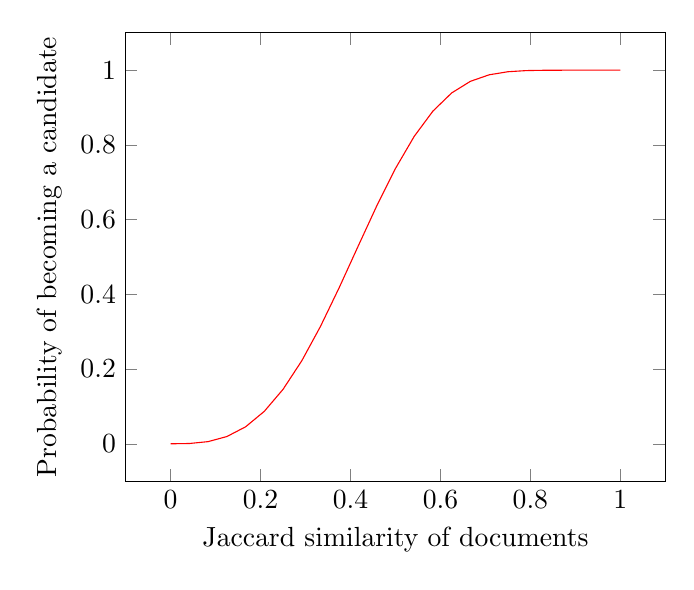
\begin{tikzpicture}
			\begin{axis}[
			xlabel = Jaccard similarity of documents,
			ylabel = Probability of becoming a candidate,
			]
			\addplot[domain=0:1,color=red]{1-(1-x^3)^10};
			\end{axis}
			\end{tikzpicture}
		}
		\item{$r=6$ and $b=20$
			
			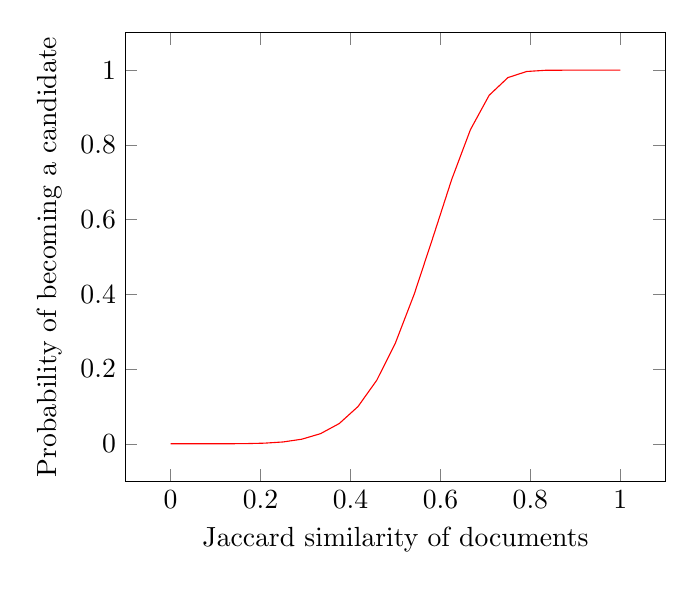
\begin{tikzpicture}
			\begin{axis}[
			xlabel = Jaccard similarity of documents,
			ylabel = Probability of becoming a candidate,
			]
			\addplot[domain=0:1,color=red]{1-(1-x^6)^20};
			\end{axis}
			\end{tikzpicture}
		}
		\item{$r=5$ and $b=50$
			
			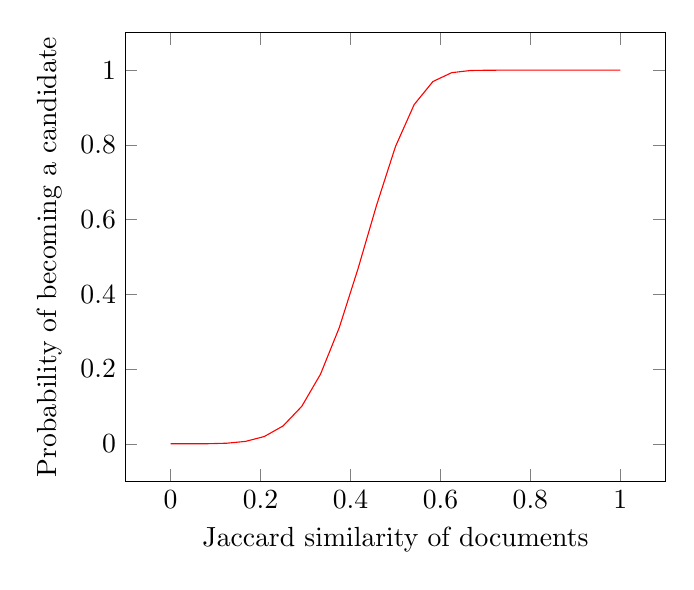
\begin{tikzpicture}
			\begin{axis}[
			xlabel = Jaccard similarity of documents,
			ylabel = Probability of becoming a candidate,
			]
			\addplot[domain=0:1,color=red]{1-(1-x^5)^50};
			\end{axis}
			\end{tikzpicture}
		}
	\end{itemize}
}

\item{For each of the $(r,b)$ pairs in (a), compute the threshold, that is, the value of $s$ for which the value of $1-(1-s^r)^b$ is exactly $1/2$. How does this value compare with the estimate of $(1/b)^{1/r}$ that was suggested in Section 3.4.2?

\begin{center}
	\begin{tabular}{ c | c | c | c }
		           & \makecell{$s$ when \\ $1-(1-s^r)^b=1/2$} & $(1/b)^{1/r}$ & $|\text{Difference}|$ \\ \hline\hline
		$r=3,b=10$ & 0.40609                                  & 0.46415       & 0.058                  \\
		$r=6,b=20$ & 0.56935                                  & 0.60696       & 0.038                  \\
		$r=5,b=50$ & 0.42439                                  & 0.45730       & 0.033
	\end{tabular}
\end{center}
}
\end{enumerate}

\section{Assignment 3: Minhashing in Java}
App.java:
\inputminted[breaklines=true]{java}{java/Exercise4Assignment3/src/main/java/com/intelligent/data/management/Exercise4Assignment3/App.java}

\end{document}
